\documentclass[12pt,a4paper,oneside]{article}

\usepackage{graphicx}
\usepackage{amsmath}
\usepackage{amsthm}
\usepackage{amssymb}
\usepackage{breqn}
\usepackage{listings}
\usepackage{xcolor}
\usepackage{textcomp}
\usepackage{setspace}
\usepackage[final]{pdfpages}
\usepackage{lscape}
\usepackage{cite}
\usepackage[toc,page]{appendix}
\usepackage{epstopdf}
\usepackage{multicol}
\usepackage[includeheadfoot, margin=2cm]{geometry}
\usepackage{fancyhdr}
\usepackage{url}
\usepackage{lscape}
\usepackage{rotating}
\usepackage{booktabs}
\usepackage{float}
\usepackage{cancel}
\usepackage[framed,numbered,autolinebreaks,useliterate]{mcode}
\usepackage[colorlinks=false,pdfborder={0 0 0}]{hyperref}
\usepackage{placeins}
\usepackage[utf8]{inputenc}
\usepackage[T1]{fontenc}
\usepackage{lmodern}

\bibliographystyle{plain}
% Figures within a column...
\makeatletter
\newenvironment{tablehere}
{\def\@captype{table}}
{}
\newenvironment{figurehere}
{\def\@captype{figure}}
{}
\makeatother

%commands
\providecommand{\e}[1]{\ensuremath{\times 10^{#1}}}

% Set figure numbering
\renewcommand{\thefigure}{\arabic{section}.\arabic{figure}}
\renewcommand{\theequation}{\arabic{section}.\arabic{equation}}
\renewcommand{\thetable}{\arabic{section}.\arabic{table}}

% Title Page
\title{\begin{figure}[!htb]
\centering

\includegraphics[width = 0.8\textwidth]{../Images/usyd.jpg}
\end{figure}
\textsc{AMME4112}\\{Work Notes}}
\vspace{10mm}
\vspace{5mm}
\author{Stephen Wardrop - 310185599}
\date{\today}

\begin{document}
\maketitle
\thispagestyle{empty}
\pagebreak

\pagenumbering{roman}
\tableofcontents
\pagebreak
\fancyhf{}
\fancyhead[L]{}
\fancyhead[R]{AMME4111 - Work Notes}
\fancyfoot[C]{\thepage}
\pagestyle{fancy}
\pagenumbering{arabic}


\section{Simulating Compass Gait Walker}\setcounter{figure}{0}\setcounter{equation}{0}\setcounter{table}{0}
\subsection{Continuous phase of walker}

\subsubsection*{Forward Kinematics}
\begin{align}
	x_1 &= \frac{l_1}{2}\cos\theta_1\nonumber \\
	\dot{x_1} &= -\frac{l_1}{2}\sin(\theta_1)\dot{\theta}_1\nonumber \\
	y_1 &= \frac{l_1}{2}\sin\theta_1\nonumber \\
	\dot{y_1} &= \frac{l_1}{2}\cos(\theta_1)\dot{\theta}_1\nonumber \\
	x_2 &= l_1\cos\theta_1 + \frac{l_2}{2}\cos(\theta_1 + \theta_2)\nonumber \\
	\dot{x_2} &= -l_1\sin(\theta_1)\dot{\theta}_1 - \frac{l_2}{2}\sin(\theta_1 + \theta_2)(\dot{\theta}_1 + \dot{\theta}_2)\label{eqn:x2dot} \\
	y_2 &= l_1\sin\theta_1 + \frac{l_2}{2}\sin(\theta_1 + \theta_2)\nonumber \\
	\dot{y_2} &= l_1\cos\theta_1\dot{\theta}_1 + \frac{l_2}{2}\cos(\theta_1 + \theta_2)(\dot{\theta}_1 + \dot{\theta}_2)\label{eqn:y2dot}
\end{align}  
\subsubsection*{Lagrangian Dynamics}
In order to produce the dynamical equations for the two-link manipulator, we must compute the Lagrangian:
\begin{align}
	L &= K - P\nonumber \\
	T_i &= \frac{\partial}{\partial{t}}\left(\frac{\partial{L}}{\partial{\dot{\theta}_i}}\right) - \frac{\partial{L}}{\partial{\theta_i}}\label{eqn:T_i}
\end{align}
The kinetic energy of the manipulator is given by the summation of the pure rotational kinetic energy of the first link about the origin and the rotational kinetic energy of the second link about its centre and the linear KE of its centre of mass.
\begin{align}
	K &= \frac{1}{2}I_1\dot{\theta}_1^2 + \frac{1}{2}I_2(\dot{\theta}_1 + \dot{\theta}_2)^2 + \frac{1}{2}m_2 V_2^2\label{eqn:KE}
\end{align}
From equations \ref{eqn:x2dot} and \ref{eqn:y2dot}, we have expressions for the components of $V_2$:
\begin{align*}
	V_2^2 &= \left[l_1^2 s_1^2 \dot{\theta}_1^2 + l_1 l_2 s_1 s_{12} \dot{\theta}_1(\dot{\theta}_1 + \dot{\theta}_2) + \frac{l_2^2}{4} s_{12}^2(\dot{\theta}_1 + \dot{\theta}_2)^2\right] \\
	& + \left[l_1^2 c_1^2 \dot{\theta}_1^2 + l_1 l_2 c_1 c_{12} \dot{\theta}_1(\dot{\theta}_1 + \dot{\theta}_2) + \frac{l_2^2}{4} c_{12}^2(\dot{\theta}_1 + \dot{\theta}_2)^2\right]
\end{align*}
Combining terms and exploiting the trigonometric identities $\sin^2{x} + \cos^2{x} = 1$ and $\cos(x - y) = \cos{x}\cos{y} + \sin{x}\sin{y}$:
\begin{align}
	V_2^2 &= l_1^2 \dot{\theta}_1^2 + l_1 l_2 c_2 \dot{\theta}_1(\dot{\theta}_1 + \dot{\theta}_2) + \frac{1}{4}l_2^2(\dot{\theta}_1 + \dot{\theta}_2)^2\label{eqn:V_2}
\end{align}
Substituting equation \ref{eqn:V_2} into equation \ref{eqn:KE}:
\begin{align}
	K =& \frac{1}{2}I_1\dot{\theta}_1^2 + \frac{1}{2}I_2\left(\dot{\theta}_1 + \dot{\theta}_2\right)^2\nonumber \\
	& + \frac{1}{2}m_2\left[\dot{\theta}_1^2\left(l_1^2 + \frac{1}{4}l_2^2 + l_1 l_2 c_2\right) + \dot{\theta}_2^2\left(\frac{1}{4}l_2^2\right) + \dot{\theta}_1\dot{\theta}_2\left(\frac{1}{2}l_2^2 + l_1 l_2 c_2\right)\right]\nonumber \\
	P =& \frac{1}{2}l_1 s_1 m_1 g + \left(l_1 s_1 + \frac{1}{2}l_2 s_{12}\right)m_2 g\nonumber \\
	L =& \frac{1}{2}\dot{\theta}_1^2 \left(I_1 + I_2 + m_2\left(l_1^2 + \frac{1}{4}l_2 + l_1 l_2 c_2 \right) \right) + \frac{1}{2}\dot{\theta}_2^2\left(I_2 + \frac{1}{4}m_2 l_2^2 \right)\nonumber \\
	& + \dot{\theta}_1\dot{\theta}_2 \left(I_2 + \frac{1}{2}m_2 \left(\frac{1}{2}l_2^2 + l_1 l_2 c_2 \right) \right) - \frac{1}{2}l_1 s_1 m_1 g - \left(l_1 s_1 + \frac{1}{2}l_2 s_{12}\right)m_2 g\label{eqn:L}
\end{align}
Now, we can determine equations for the torques using equations \ref{eqn:T_i} and \ref{eqn:L}.
\begin{align*}
	\frac{\partial{L}}{\partial{\dot{\theta}_1}} =& \dot{\theta}_1\left(I_1 + I_2 + m_2 \left(l_1^2 + \frac{1}{4}l_2^2 + l_1 l_2 c_2 \right) \right) + \dot{\theta}_2 \left(I_2 + \frac{1}{2}m_2 \left(\frac{1}{2}l_2^2 + l_1 l_2 c_2 \right) \right) \\
	\frac{\partial}{\partial{t}}\left(\frac{\partial{L}}{\partial{\dot{\theta}_1}}\right) =& \ddot{\theta}_1 \left(I_1 + I_2 + m_2\left(l_1^2 + \frac{1}{4}l_2^2 + l_1 l_2 c_2 \right) \right) - \dot{\theta}_1 \dot{\theta}_2 \left(m_2 l_1 l_2 s_2 \right) \\
	&+ \ddot{\theta}_2 \left(I_2 + \frac{1}{2}m_2\left(\frac{1}{2}l_2^2 + l_1 l_2 c_2 \right)\right) - \dot{\theta}_2^2 \left( \frac{1}{2} m_2 l_1 l_2 s_2 \right) \\
	\frac{\partial{L}}{\partial{\theta_1}} =& -\frac{1}{2}l_1 c_1 m_1 g - m_2 g \left(l_1 c_1 + \frac{1}{2}l_2 c_{12} \right)
\end{align*}
Adding the components together, we get:
\begin{align}
	T_1 =& \ddot{\theta}_1 \left(I_1 + I_2 + m_2\left(l_1^2 + \frac{1}{4}l_2^2 + l_1 l_2 c_2 \right) \right) - \dot{\theta}_1 \dot{\theta}_2 \left(m_2 l_1 l_2 s_2 \right)\nonumber \\
	&+ \ddot{\theta}_2 \left(I_2 + \frac{1}{2}m_2\left(\frac{1}{2}l_2^2 + l_1 l_2 c_2 \right)\right) - \dot{\theta}_2^2 \left( \frac{1}{2} m_2 l_1 l_2 s_2 \right)\nonumber \\
	&+ \frac{1}{2}l_1 c_1 m_1 g + m_2 g \left(l_1 c_1 + \frac{1}{2}l_2 c_{12} \right)\label{eqn:T1}
\end{align}
Likewise for $T_2$:
\begin{align*}
	\frac{\partial{L}}{\partial{\dot{\theta}_2}} =& \dot{\theta}_2 \left(I_2 + \frac{1}{4}m_2 l_2^2 \right) + \dot{\theta}_1 \left(I_2 + \frac{1}{2}m_2 \left(\frac{1}{2}l_2^2 + l_1 l_2 c_2 \right) \right) \\
	\frac{\partial}{\partial{t}}\left(\frac{\partial{L}}{\partial{\dot{\theta}_2}}\right) =& \ddot{\theta}_2\left(I_2 + \frac{1}{4}m_2 l_2^2 \right) + \ddot{\theta}_1\left(I_2 + \frac{1}{2}m_2 \left(\frac{1}{2}l_2^2 + l_1 l_2 c_2 \right) \right) - \dot{\theta}_1 \dot{\theta}_2 \left(\frac{1}{2}m_2 l_1 l_2 s_2 \right) \\
	\frac{\partial{L}}{\partial{\theta_2}} =& - \dot{\theta}_1^2 \left(\frac{1}{2}m_2 l_1 l_2 s_2 \right) - \dot{\theta}_1\dot{\theta}_2 \left(\frac{1}{2} m_2 l_1 l_2 s_2 \right) - \frac{1}{2} m_2 g l_2 c_{12}
\end{align*}
Adding components as for $T_1$:
\begin{align}
	T_2 =& \ddot{\theta}_2\left(I_2 + \frac{1}{4}m_2 l_2^2 \right) + \ddot{\theta}_1\left(I_2 + \frac{1}{2}m_2 \left(\frac{1}{2}l_2^2 + l_1 l_2 c_2 \right) \right)\nonumber \\
	&+ \dot{\theta}_1^2 \left(\frac{1}{2}m_2 l_1 l_2 s_2 \right) + \frac{1}{2} m_2 g l_2 c_{12}\label{eqn:T2}
\end{align}

Thus we have an equation of the form
\begin{equation}
	M\left(q(t)\right)\ddot{q}(t) + C\left(q(t),\dot{q}(t)\right)\dot{q}(t)
	 + G\left(q(t)\right) = B\left(q(t)\right)u(t)
\end{equation} where
\begin{eqnarray*}
	M\left(q(t)\right) &=& \begin{bmatrix}
		I_1 + I_2 + m_2\left(l_1^2 + \frac{1}{4}l_2^2 + l_1l_2\cos{q_2}\right) &
		I_2 + \frac{1}{2}m_2\left(\frac{1}{2}l_2^2 + l_1l_2\cos{q_2}\right) \\
		I_2 + \frac{1}{2}m_2\left(\frac{1}{2}l_2^2 + l_1l_2\cos{q_2}\right) &
		I_2 + \frac{1}{4}m_2l_2^2
	\end{bmatrix} \\
	C\left(q(t),\dot{q}(t)\right) &=& \begin{bmatrix}
		-m_2 l_1 l_2 \sin({q_2}) \dot{q}_2 &
		-\frac{1}{2}m_2 l_1 l_2 \sin({q_2}) \dot{q}_2 \\
		\frac{1}{2}m_2 l_1 l_2 \sin({q_2}) \dot{q}_1 & 0
	\end{bmatrix} \\
	G\left(q(t)\right) &=& \begin{bmatrix}
		\frac{1}{2}l_1 \cos{q_1} m_1 g + m_2 g \left(l_1 \cos{q_1} + \frac{1}{2}l_2 \cos{(q_1 + q_2)} \right) \\
		\frac{1}{2} m_2 g l_2 \cos{(q_1 + q_2)}
	\end{bmatrix} \\
	B\left(q(t)\right) &=& \begin{bmatrix}
		0 \\ 1
	\end{bmatrix}, ~
	u(t) = T_2, ~
	q(t) = \begin{bmatrix}
		q_1(t) \\ q_2(t)
	\end{bmatrix}
\end{eqnarray*}

\subsection{Impact dynamics}
Following the derivation as presented by Westervelt \cite{westervelt2007feedback}, the full-state impact dynamics are of the form: \\
\begin{eqnarray}
	q\left(t^+\right) &=& Rq\left(t^-\right) \\
	\dot{q}\left(t^+\right) &=& R\Delta\left(q\left(t^-\right)\right)\dot{q}\left(t^-\right)
\end{eqnarray}

The condition for impact for walking on flat ground is $\theta_2 = -2 \theta_1$ AND $\theta_2 < -180 + \epsilon$, where $\epsilon$ is chosen such that the shortest footstep is possible. The second condition assumes that it is not possible to step backwards. This is reasonable, since the current objective is to construct feasible forward-walking motion. \\ \par

\begin{figure}[htp]
	\centering
	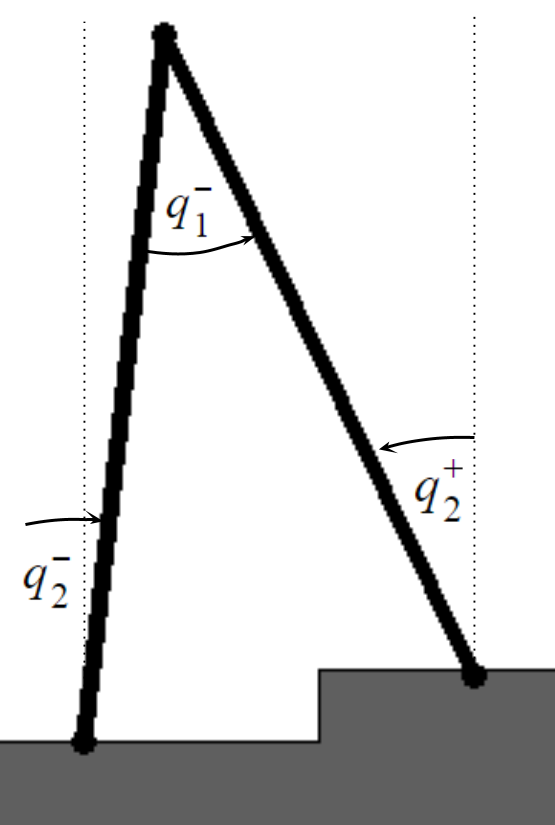
\includegraphics[scale=1]{../images/impact.png}
	\caption{Change of coordinates at impact}
	\label{fig:changecoords}
\end{figure}

The change of coordinates at impact is depicted in Figure~\ref{fig:changecoords}. It can be trivially shown that $\theta_1^* = \pi - \theta_1$ and that $\theta_2^* = 2\pi - \theta_2$. In order to find the derivatives of $\theta_1^*$ and $\theta_2^*$, we examine the general form of these angles (i.e. at non-specific angle values). It is not difficult to derive that $\theta_1^* = \theta_1 + \theta_2 + \pi$ and it is noted that $\theta_2^* = 2\pi - \theta_2$ in general. Thus $\dot{\theta}_1^* = \dot{\theta_1} + \dot{\theta}_2$ and $\dot{\theta}_2^* = -\dot{\theta}_2$. \\

If we assume that angular momentum is conserved, i.e. $L^+ = L^-$, where
\begin{eqnarray*}
	L^- &=& I_1\dot{\theta}_1 + I_2\left(\dot{\theta}_1 + \dot{\theta}_2\right) \\
	L^+ &=& I_1\dot{\theta}_1^* + I_2\left(\dot{\theta}_1^* + \dot{\theta}_2^*\right)
\end{eqnarray*}
\par Substituting values for $\dot{\theta}_1^*$ and $\dot{\theta}_2^*$, we get
\begin{equation}
	\dot{\theta}_1^+\left(I_1 + I_2\right) + \dot{\theta}_2^+\left(I_1\right)
	= \dot{\theta}_1^-\left(I_1 + I_2\right) + \dot{\theta}_2^-\left(I_2\right)
\end{equation}
This equation does not yet yield a solution for $\theta_1^+, \theta_2^+$, since we at this stage need one to find the other.
\pagebreak

\section{Virtual Holonomic Constraints}\setcounter{figure}{0}\setcounter{equation}{0}\setcounter{table}{0}
A viable virtual holonomic constraint is one which can guarantee feasible motion of the robotic walker given some reasonable initial conditions. A favourable condition for a family of virtual constraints is that they are able to be sparsely identified and can be classified by at least a partial ordering. For simplicity, it is also desirable that the constraints are time-invariant.

\subsection{Simple linear constraints}
The constraint for keeping the end of the swing leg at the same level as the end of the stance leg is
\begin{equation}
	\theta_2 = -2\theta_1
\end{equation}
for the coordinate system chosen. This constraint can generate feasible walking, but cannot account for the energy lost in collisions, and does not comply with the assumption made of the hybrid zero dynamics being invariant. In the general case, it is not straightforward to use linear constraints to set a desired end position, and the range of motion is strictly limited. As a result, linear constraints should not be chosen as a basis for the library of motion primitives.

\subsection{Bézier curve constraints}
Bézier curves provide a way to produce families of curves for particular start and end heights and are sparsely identified by only $n+1$ points, where $n$ is the degree of the curve. These points provide an intuitive way of defining the curve, in contrast with polynomial coefficients.
\par

Theoretically, these curves need only be defined from the start to the endpoint of the continuous-phase which they specify. However, since the curve provides a virtual constraint to be enforced by a controller, it is necessary to define the curve over the full range of possible motion, here considered to be $\theta_1 \in \left[0, \pi\right]$, else it is possible for the walker to enter a region where the control signal is undefined. If we assume that the overshoot past the desired endpoint is small, then the shape of the curve should be flat outside the defined region. That is, when we leave the target region, we wish to set $\theta_2$ to the closest defined $\theta_2$. \\ \par

For the compass-gait walker, a general Bézier curve is defined by the following parametric equation.
\begin{equation}
	\begin{bmatrix}
		\theta_1 \\ \theta_2
	\end{bmatrix}
	=
	\sum_{i=0}^{n}\binom{n}{i}\left(1-t\right)^{n-i}t^i
	\begin{bmatrix}
		\theta_{1_i} \\ \theta_{2_i}
	\end{bmatrix} \label{eqn:genBez}
\end{equation}
Since this equation is not monotonic in $\theta_1$, it is not a convenient expression. Therefore, we build families of Bézier curves with the following formulation:
\begin{eqnarray}
	t &=& \frac{\theta_1 - \theta_{1_0}}{\theta_{1_n} - \theta_{1_0}} \\
	\theta_2 &=& \sum_{i=0}^{n}\binom{n}{i}\left(1-t\right)^{n-i}t^i\theta_{2_i}
\end{eqnarray}
This is expressible explicitly as
\begin{equation}
	\theta_2 = \frac{1}{\left(\theta_{1_n} - \theta_{1_0}\right)^n}\sum_{i=0}^{n}\binom{n}{i}
		\left(\theta_{1_n} - \theta_1\right)^{n-i}
		\left(\theta_1 - \theta_{1_0}\right)^i\theta_{2_i} \label{eqn:expBez}
\end{equation}
This formulation removes our ability to arbitrarily define the control points $\left(\theta_{1_i}, \theta_{2_i}\right)$, other than the endpoints. That is, this formulation produces curves of the form given in Equation~\ref{eqn:genBez} with
\begin{equation}
	\theta_{1_i} = \frac{i}{n}\left(\theta_{1_n}-\theta_{1_0}\right) + \theta_{1_0} ~~
	\forall ~~ i \in \left[1,~n-1\right]
\end{equation}

Since we can only define one of the two variables in each control point, to yield arbitrary curves of order $n$, before achievable with $n - 1$ free control points (i.e. non-endpoint control points), now requires $2n - 2$ such points. Since it is desirable to have the ability to set the gradient of approach to the control points independently of the shape of the polynomial (achievable using a general cubic Bézier curve) we use a quintic curve in the new formulation. This requires six control points. \\ \par

As in \cite{manchester13planning}, assume the hybrid zero dynamics are invariant, then:
\begin{eqnarray}
	\theta^+ &=& \kappa \\
	\dot{\theta}^+ &=& \delta\dot{\theta}^-
\end{eqnarray}
when $\theta = \theta_f$. Note that $\theta^+$ is fixed by the specification of the constraint. I need to understand what this $\delta$ is.\\ \par
\pagebreak

\section{Partial Closed-Form Solutions for Velocity and Energy}
\setcounter{figure}{0}\setcounter{equation}{0}\setcounter{table}{0}
As in \cite{manchester13planning}, we produce functions of the form
\begin{equation}
	\alpha\left(\theta\right)\ddot{\theta}(t) + \beta\left(\theta\right)\dot{\theta}(t)^2 + \gamma\left(\theta\right) = 0
\end{equation}
with
\begin{eqnarray*}
	\alpha(\theta) &=& B^{\bot}\left(\Phi(\theta)\right)M\left(\Phi(\theta)\right)\Phi'(\theta)\\
	\beta(\theta) &=& B^{\bot}\left(\Phi(\theta)\right)\left(M\left(\Phi(\theta)\right)\Phi''(\theta)
		+C\left(\Phi(\theta),\Phi'(\theta)\right)\Phi'(\theta) \right)\\
	\gamma(\theta) &=& B^{\bot}\left(\Phi(\theta)\right)G\left(\Phi(\theta)\right)\\
\end{eqnarray*}
Then we get the differential equation:
\begin{equation} \label{eqn:diff}
	\frac{d}{d\theta}{\dot{\theta}\left(\theta\right)}^2 = -2\frac{\beta\left(\theta\right)}
	{\alpha\left(\theta\right)}\dot{\theta}\left(\theta\right)^2 - 2\frac{\gamma\left(\theta\right)}
	{\alpha\left(\theta\right)}
\end{equation}

Solving this over any interval $\theta \in \left[\theta_0,\theta_f\right]$ yields
\begin{equation} \label{eqn:affine}
	\dot{\theta}\left(\theta\right)^2 = \Gamma\left(\theta,\theta_0\right)\dot{\theta}^2 
	+ \Psi\left(\theta, \theta_0\right)
\end{equation}

This solution is achieved by using the general method for first-order linear ODEs with varying coefficients, i.e. given
\begin{equation*}
	y'(x) + f(x)y(x) = g(x)
\end{equation*}
the solution is
\begin{equation*}
	y = e^{-\int f(x)dx}\left(\int g(x)e^{\int f(x)dx}dx + \kappa\right)
\end{equation*}
Thus we have
\begin{eqnarray}
	\Gamma(\theta) &=& e^{-\int_{\theta_0}^{\theta}f(x)dx} \\
	\Psi(\theta) &=& e^{-\int_{\theta_0}^{\theta}f(x)dx}
		\int_{\theta_0}^{\theta}g(x)e^{\int_{\theta_0}^{\theta}f(x)dx} \\
	f(x) &=& 2\frac{\beta(x)}{\alpha(x)} \nonumber \\
	g(x) &=& -2\frac{\gamma(x)}{\alpha(x)} \nonumber
\end{eqnarray}

The total mechanical energy of the system is given by
\begin{equation}
	\bar{H}\left(\theta,\dot{\theta}\right) = \Phi'\left(\theta\right)^T M\left(\Phi\left(\theta\right)\right)
	\Phi'\left(\theta\right)\dot{\theta}^2 + V\left(\Psi\left(\theta\right)\right)
\end{equation}
Where M is the symmetric, positive-definite mass/inertia matrix and
\begin{eqnarray*}
	\Phi\left(\theta\right) &=& \left[ q_1, q_2, \ldots, q_n \right]^T \\
	&=& \left[ \phi_1\left(\theta\right), \phi_2\left(\theta\right), \ldots, \phi_n\left(\theta\right)
	\right]^T \\
	\Phi'\left(\theta\right) &=& \left[ \frac{\partial\phi_1\left(\theta\right)}{\partial\theta},
	\frac{\partial\phi_2\left(\theta\right)}{\partial\theta}, \ldots ,
	\frac{\partial\phi_n\left(\theta\right)}{\partial\theta} \right]^T
\end{eqnarray*}

\subsection{Compass Gait with Bézier constraint}
In the case of the compass-gait walker, of course, since there is only one variable other than the phase variable $\theta$, these functions have only two elements each, one of which is trivial. Thus:
\begin{eqnarray*}
	\Phi\left(\theta\right) &=& 
		\begin{bmatrix}
		\theta \\ \phi\left(\theta\right)
		\end{bmatrix} \\
	\Phi'\left(\theta\right) &=& 
		\begin{bmatrix}
		1 \\ \frac{\partial\phi\left(\theta\right)}{\partial\theta}
		\end{bmatrix} \\
	\Phi''\left(\theta\right) &=& 
		\begin{bmatrix}
		0 \\ \frac{\partial^2\phi\left(\theta\right)}{\partial\theta^2}
		\end{bmatrix}
\end{eqnarray*}
Now, we have from Equation~\ref{eqn:expBez} (slightly adapted to suit new coordinate naming):
\begin{equation}
	\phi\left(\theta\right) = \frac{1}{\left(\theta_f-\theta_{0}\right)^n}\sum_{i=0}^{n}\binom{n}{i}
	\left(\theta_f - \theta\right)^{n-i}
	\left(\theta - \theta_{0}\right)^i\vartheta_{i}
\end{equation}
The derivative is
\begin{dmath}
	\frac{\partial\phi}{\partial\theta} = \frac{1}{\left(\theta_f-\theta_0\right)^n}
	\left(
	{n\left( \left(\theta-\theta_0\right)^{n-1}\vartheta_n - 
		\left(\theta_f-\theta\right)^{n-1}\vartheta_0 \right) }
	+ {\sum_{i=1}^{n-1} \binom{n}{i} \left(i\left(\theta_f-\theta\right)^{n-i}
		\left(\theta-\theta_0\right)^{i-1} - 
		\left(n - i\right)\left(\theta_f-\theta\right)^{n-i-1}\left(\theta-
		\theta_0\right)^{i}\right)\vartheta_i}
	\right)
\end{dmath}
The second derivative is
\begin{dmath}
	\frac{\partial^2\phi}{\partial\theta^2} = 
	\frac{1}{(\theta_f-\theta_0)^n}
	\left(
	n(n-1)\left[ (\theta_f-\theta)^{n-2}\vartheta_0 
		+ (\theta-\theta_0)^{n-2}\vartheta_n
	+ (n-2)\left((\theta-\theta_0)(\theta_f-\theta)^{n-3}\vartheta_1
		+ (\theta_f-\theta)(\theta-\theta_0)^{n-3}\vartheta_{n-1} \right)
		- 2\left((\theta_f-\theta)^{n-2}\vartheta_1
		+ (\theta-\theta_0)^{n-2}\vartheta_{n-1} \right) 		\right]
	+ \sum_{i=2}^{n-2} \binom{n}{i} 
		\left({i(i-1)(\theta_f-\theta)^{n-i}(\theta-\theta_0)^{i-2}
			- 2i(n-i)(\theta_f-\theta)^{n-i-1}(\theta-\theta_0)^{i-1}}
			+ (n-i-1)(n-i)(\theta_f-\theta)^{n-i-2}(\theta-\theta_0)^{i} \right)
			\vartheta_i
	\right)
\end{dmath}

Let us choose the simplest non-zero $B^{\bot}$:
\begin{equation*}
	B^{\bot}=\begin{bmatrix} 1 & 0 \end{bmatrix}
\end{equation*}
We also have the following. Note that for simplicity, $\phi(\theta) = \phi$.
\begin{eqnarray*}
	M\left(\Phi(\theta)\right) &=& \begin{bmatrix}
		I_1 + I_2 + m_2\left(l_1^2 + \frac{1}{4}l_2^2 + l_1l_2\cos{\phi}\right) &
		I_2 + \frac{1}{2}m_2\left(\frac{1}{2}l_2^2 + l_1l_2\cos{\phi}\right) \\
		I_2 + \frac{1}{2}m_2\left(\frac{1}{2}l_2^2 + l_1l_2\cos{\phi}\right) &
		I_2 + \frac{1}{4}m_2l_2^2
	\end{bmatrix} \\
	C\left(\Phi(\theta),\Phi'(\theta)\right) &=& \sin({\phi}) \begin{bmatrix}
		-m_2 l_1 l_2 \frac{\partial\phi}{\partial\theta} &
		-\frac{1}{2}m_2 l_1 l_2 \frac{\partial\phi}{\partial\theta} \\
		\frac{1}{2}m_2 l_1 l_2  & 0
	\end{bmatrix} \\
	G\left(\Phi(\theta)\right) &=& \begin{bmatrix}
		\frac{1}{2}l_1m_1g\cos{\theta} + m_2 g \left(l_1 \cos{\theta} + 
		\frac{1}{2}l_2 \cos{\left(\theta + \phi\right)} \right) \\
		\frac{1}{2} m_2 g l_2 \cos{\left(\theta + \phi\right)}
	\end{bmatrix}
\end{eqnarray*}
\pagebreak

\section{Energy Heuristic}
\setcounter{figure}{0}\setcounter{equation}{0}\setcounter{table}{0}
\subsection{Best-First Search without heuristic}

\subsection{Simple heuristic currently in use}

\subsection{Improvements to heuristic}

\pagebreak
\bibliography{../references}

\end{document}
